\documentclass{article}
\usepackage{amsmath}
\usepackage{color,pxfonts,fix-cm}
\usepackage{latexsym}
\usepackage[mathletters]{ucs}
\DeclareUnicodeCharacter{32}{$\ $}
\usepackage[Calibri,T1]{fontenc}
\usepackage[utf8x]{inputenc}
\usepackage{pict2e}
\usepackage{wasysym}
\usepackage[english]{babel}
\usepackage{tikz}
\pagestyle{empty}
\usepackage[margin=0in,paperwidth=612pt,paperheight=792pt]{geometry}
\begin{document}
\definecolor{color_29791}{rgb}{0,0,0}
\begin{tikzpicture}[overlay]\path(0pt,0pt);\end{tikzpicture}
\begin{picture}(-5,0)(2.5,0)
\put(57.024,-72.34003){\fontsize{11.04}{1}\usefont{T1}{ptm}{m}{n}\selectfont\color{color_29791}W}
\put(66.864,-72.34003){\fontsize{11.04}{1}\usefont{T1}{ptm}{m}{n}\selectfont\color{color_29791}o}
\put(72.73728,-72.34003){\fontsize{11.04}{1}\usefont{T1}{ptm}{m}{n}\selectfont\color{color_29791}rkflo}
\put(93.37104,-72.34003){\fontsize{11.04}{1}\usefont{T1}{ptm}{m}{n}\selectfont\color{color_29791}w}
\put(101.3,-72.34003){\fontsize{11.04}{1}\usefont{T1}{ptm}{m}{n}\selectfont\color{color_29791} }
\put(57,-446.7){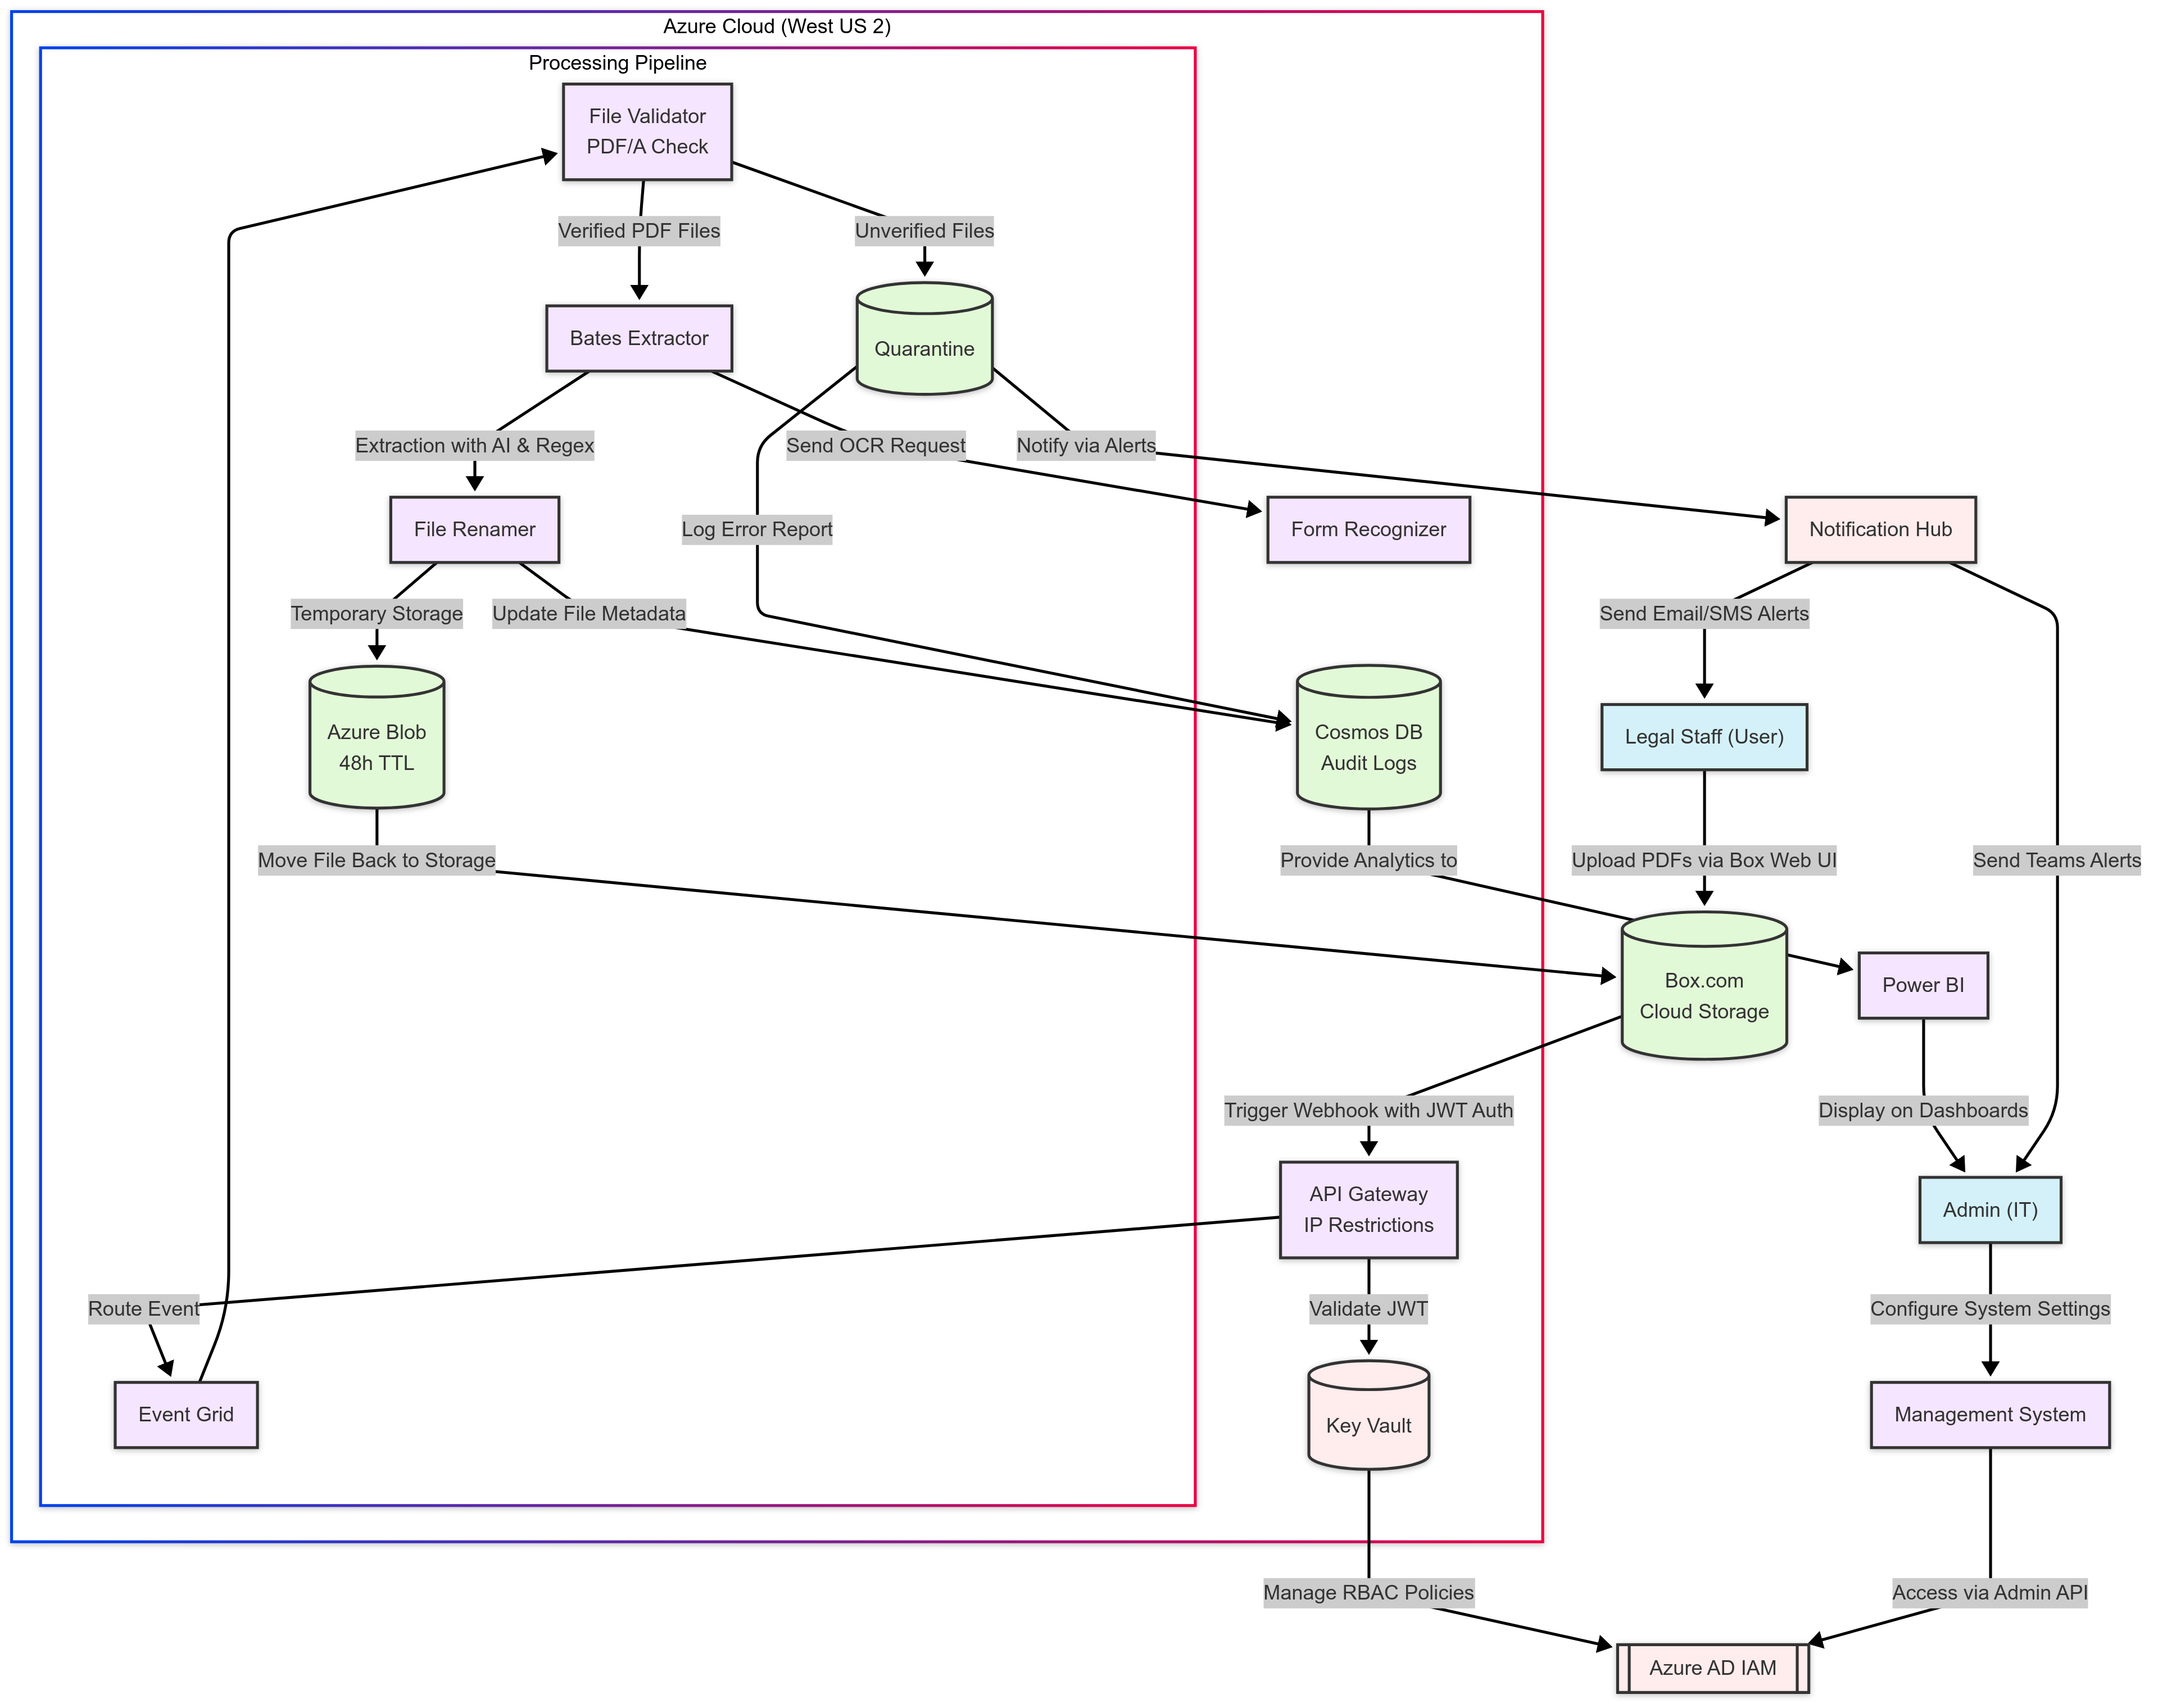
\includegraphics[width=468pt,height=370.3pt]{workflow.png}}
\put(525.1,-446.79){\fontsize{11.04}{1}\usefont{T1}{ptm}{m}{n}\selectfont\color{color_29791} }
\end{picture}
\end{document}